\section{Braking Module}

The Braking module implements the design specified in Sec.\ \ref{sec:Braking-Module-Design}. The hardware and software aspects of this module's implementation are discussed in this section.

\begin{figure}[h]
\centering
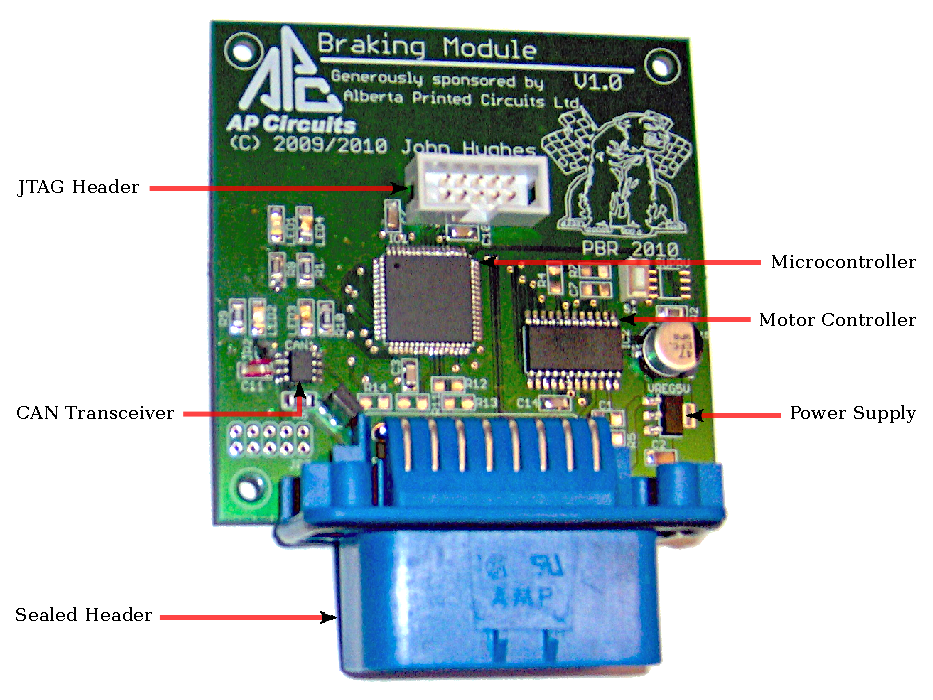
\includegraphics[scale=1]{implementation/figures/braking_pcb}
\caption{Populated Braking module PCB.}
\label{fig:braking_pcb}
\end{figure}

\subsection{Hardware}

The braking module implementation was the simplest of the 4 modules in terms of electrical design. Only one special hardware component was required, namely the stepper motor driver. This is summarized in Table \ref{table:braking_module_components}.

Figure \ref{fig:braking_pcb} shows a photograph of the completed braking module circuit board, with all components soldered on. The simplicity of the electrical design is reflected in the fact that no additional corrections (other than for the CAN transceiver) were required for the module to be 100\% operational.

\begin{table}
  \caption{Braking module components.\label{table:braking_module_components}}
  \centering
  \begin{tabular}{|c|c|c|}
    \hline 
    Part & Manufacturer & Part Number\tabularnewline 
    \hline \hline
    Stepper Motor Controller/Driver & Allegro Microsystems & A3967 \tabularnewline
    \hline
  \end{tabular}
\end{table}

\subsubsection{Stepper Motor Driver}

In order to meet the design goal of having the implementation be flexible in terms of which stepper motor would be used in the system, a current-sensing stepper motor controller/driver component was used in the circuit design. The current sense capability allows us to fix the input voltage in the circuit design, and afterwards adjust the current drive by changing resistor values in the current-sense feedback loop. 

The A3967 ``Micro-stepping Driver with Translator'' was chosen to drive the stepper motor for several reasons. The A3967 integrates a micro-stepping controller with dual H-Bridge output stages into one package. This simplified the potential circuit design. The H-Bridge output transistors can supply up to $\pm\unit{750}{\milli\ampere}$ of current at up to \unit{30}{\volt} \cite{A3967}. 

\paragraph{Current Control}
\nomenclature{$R_{sense}$}{Value of the current sense resistors in the Braking Module's stepper motor circuit.}
\nomenclature{$I_{TRIP}max$}{Maximum current allowed to flow into the Braking Module's stepper motor before the PWM circuit shuts the output stage off.}

The current control feature of the A3967 works by sensing the current through a sense resistor, $R_{sense}$, and varies the duty cycle of a fixed off-time PWM circuit, which controls the output from the H-Bridge stages.

The value of the sense resistor was determined by an equation recommended in the datasheet:
\begin{equation}
R_{sense}=\frac{0.5}{I_{TRIP}max}
\end{equation}
where $I_{TRIP}max$ is the maximum current allowed to flow into the motor before the PWM circuit shuts the output stage off.

The actual value of $R_{sense}$ used for bench testing the Braking module was \unit{2}{\ohm}, which allows \unit{250}{\milli\ampere} output current. This was suitable for the stepper motor used in testing.

\subsubsection{Analogue-to-Digital Converter}

The AT90CAN128's built-in analogue-to-digital converter was used to measure the analogue signals from the brake pressure transducers.

\subsubsection{End-of-Travel Microswitches}



\subsection{Software}


\subsubsection{Bias Library}


\paragraph{Bias Position Request}

<Position request flow chart>


\paragraph{Bias Calibration}

<Calibration flow chart>


\subsubsection{Pressure Library}


\paragraph{Periodic Pressure Output}


\paragraph{Pressure Calibration}

<Calibration flow chart>


\subsubsection{CAN Interface}

<Data flow diagram>


\subsubsection{Main Control Loop}